\section{Model 3}

The results displayed in this section are for the uncertainty involved in the calculation of flamespeed depending  on two parameter i.e the activation energy for the fall off reaction in the ozone mechanism and the pre exponential factor for third reaction in the mechanism. The percentage of ozone is taken as 40, 46, 53, 75, and 100  percent acccording to the experimental data available to us from Streng\cite{Streng}.The results are displayed in four sections. In first section, for constant surrogate size, the number of samples are changed from 1e7 to 9e7 and convergence is observed. In the second part of the results, convergence study is done for surrogates with different sizes. In third section, we ensure that samples of the parameter which we are drawing are fitting the flamespeed values of the experiment. In the fourth section mean and correlation plots are shown for the samples of both the parameters. The surrogates for individual concentrations are constructed using linear interpolation function. The initial guess for the map point is calculated using nelder mead optimization technique. After supplying initial guess over large domain it is found that the map point is the same no matter where we start our guess. 


 In this section, we display results for sample size 1e7 and surrogate of 100*100 points. We  have plotted the kde. 

\begin{figure}[H]
\subfloat[KDE \label{subfig-4:KDE for $A_3$}]{
        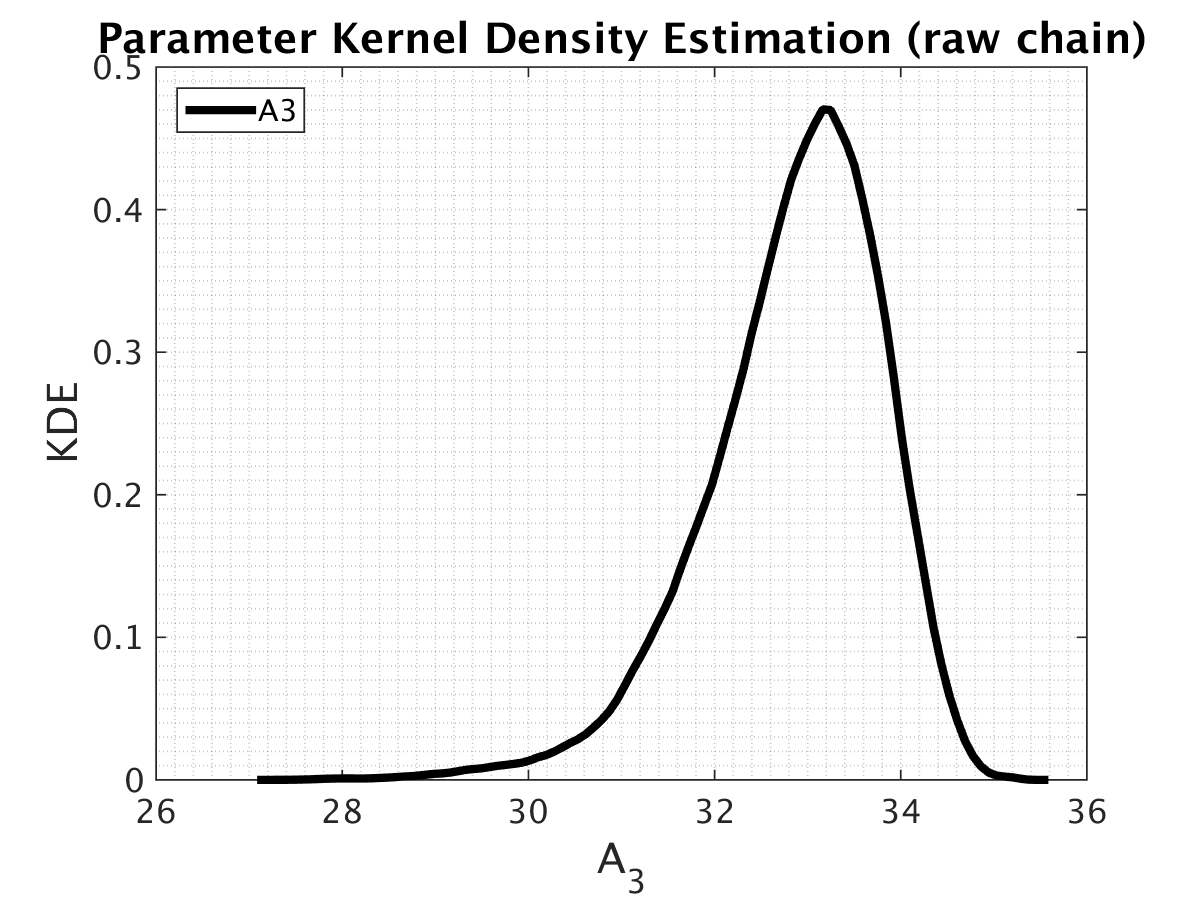
\includegraphics[scale=0.45]{model_3/kde_1} 
            }             
\subfloat[KDE \label{subfig-4:KDE for $E_3$}]{
        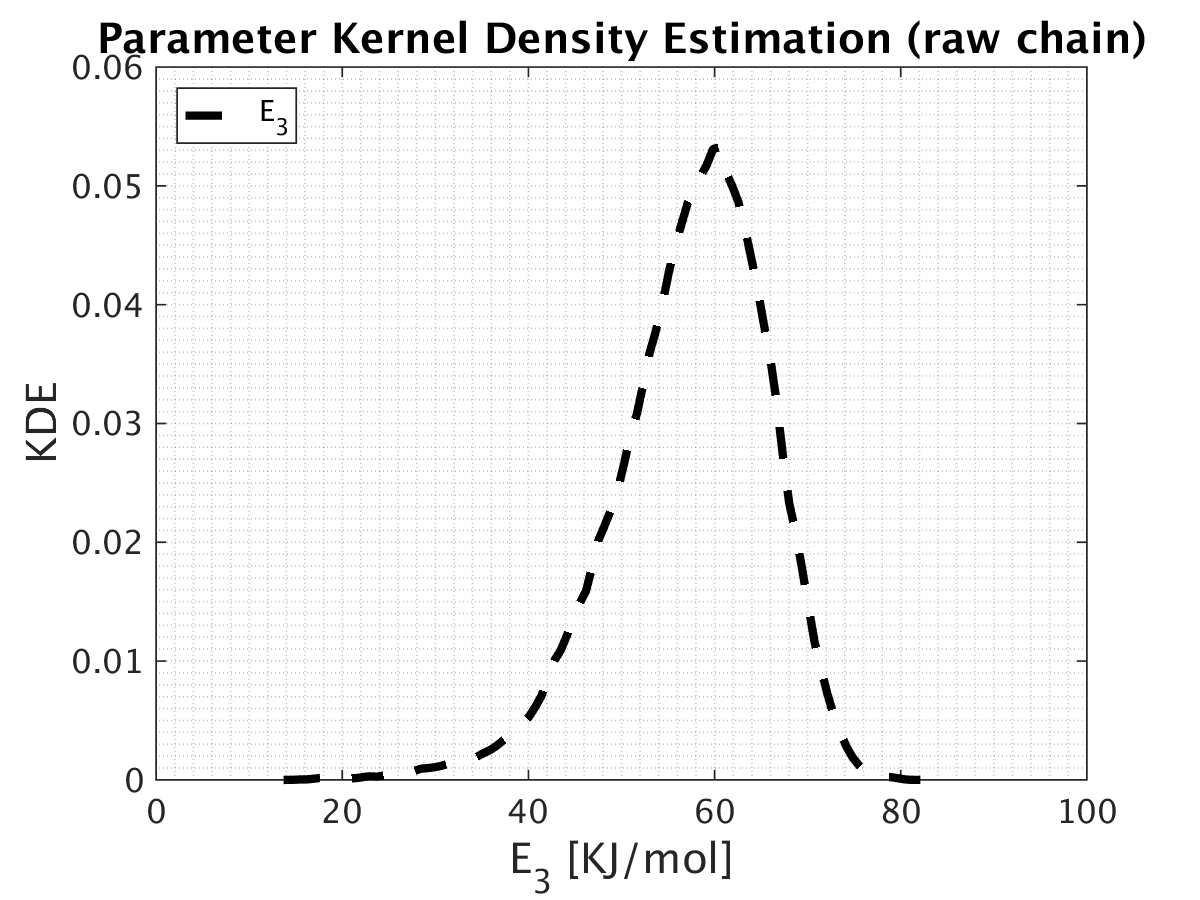
\includegraphics[scale=0.45]{model_3/kde_2} 
            }  
    \caption{Results for sample size 1e7}
\end{figure}


\subsection{Convergence Study- Number of samples }

 In this section, we see the convergence of the probability distribution as we increase the raw chain sample size. The plot is done for surrogate size of 100. In this analysis, raw chain size of $1e5$, $5e5$ , $1e6$, $5e6$ and $1e7$ is taken. 

\begin{figure}[H]
\subfloat[$A_3$ sample convergence \label{subfig-4:samp for $A_3$}]{
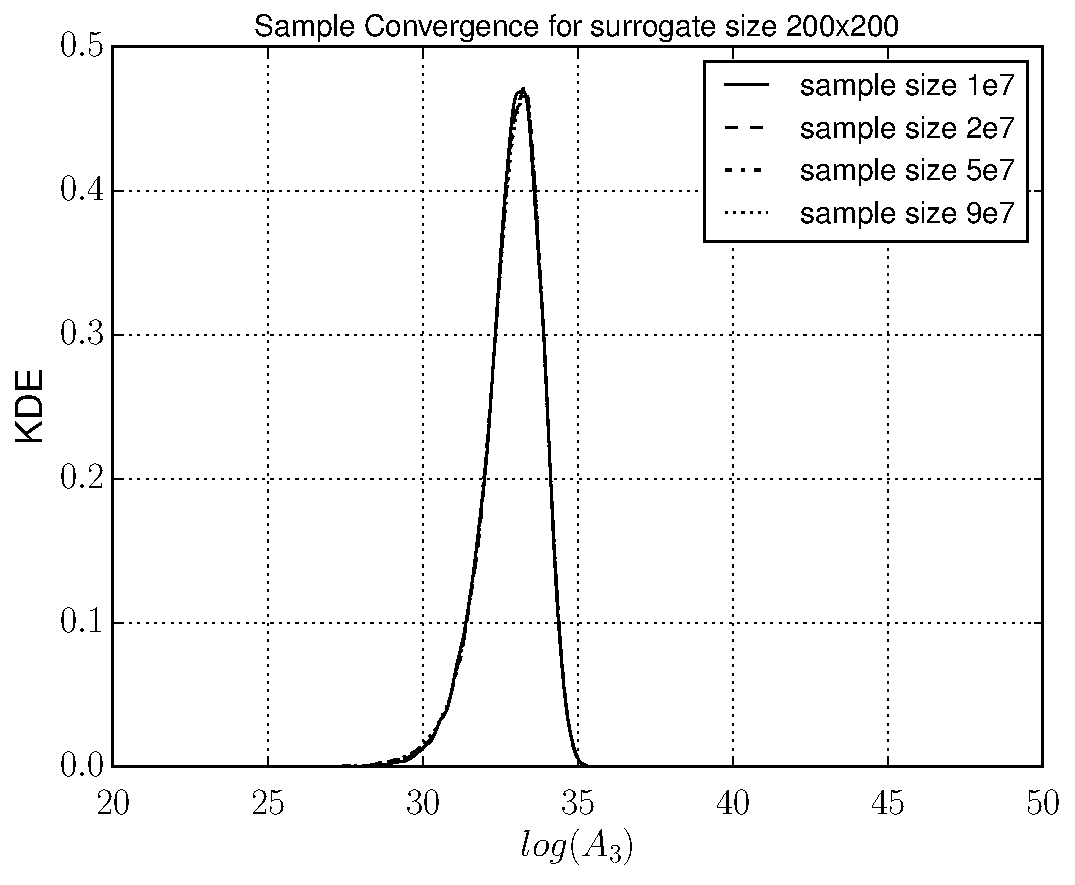
\includegraphics[scale = 0.45]{model_3/sample_conv_A3.pdf} 
}
\subfloat[$E_3$ sample convergence \label{subfig-4:samp for $E_3$}]{
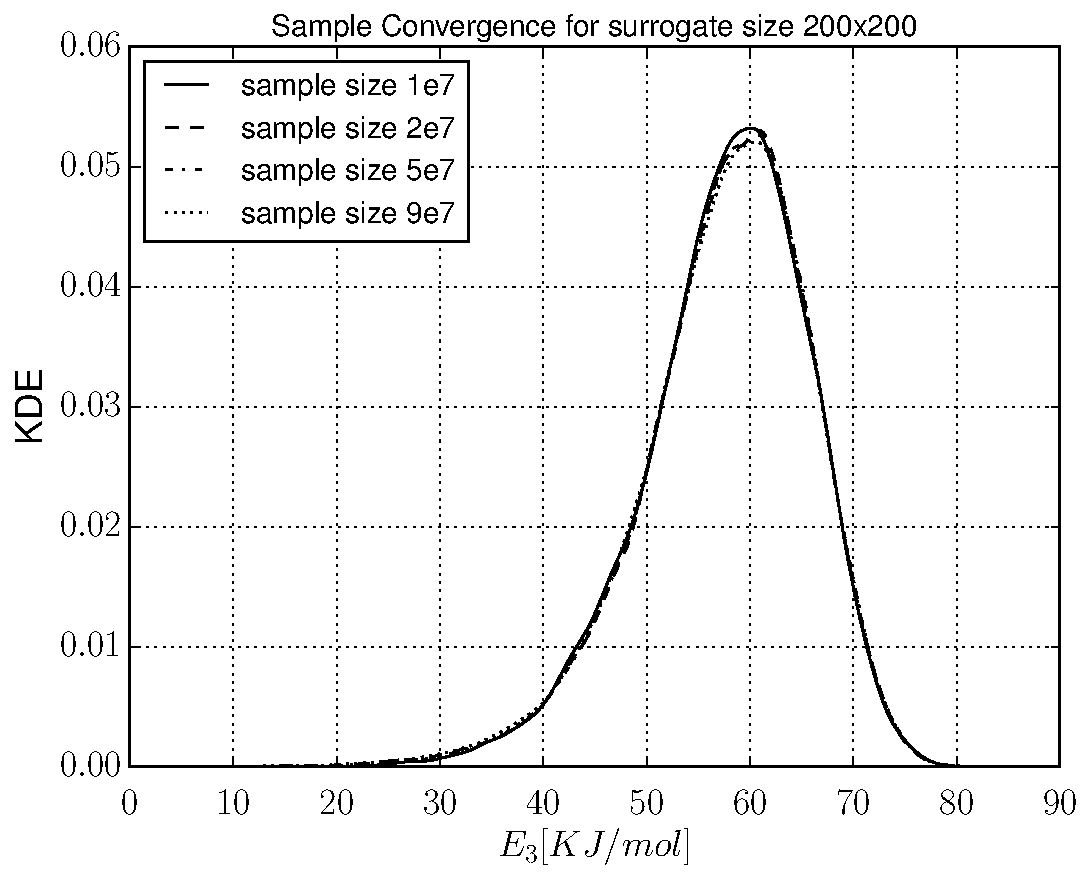
\includegraphics[scale = 0.45]{model_3/sample_conv_E3.pdf} 
}
    \caption{Convergence for surrogate size 200x200}
\end{figure}


\subsection{Convergence Study- Surrogate }

 In this section, we see the convergence of the surrogate. As we increase the number of points in the surrogate, results should be close for different surrogate sizes. The plot is done for surrogate size of 75, 100, 150, and 200. In this analysis, raw sample chain size is $1e7$. 

\begin{figure}[H]
\subfloat[$A_3$ surrogate convergence \label{subfig-5:surr for $A_3$}]{
			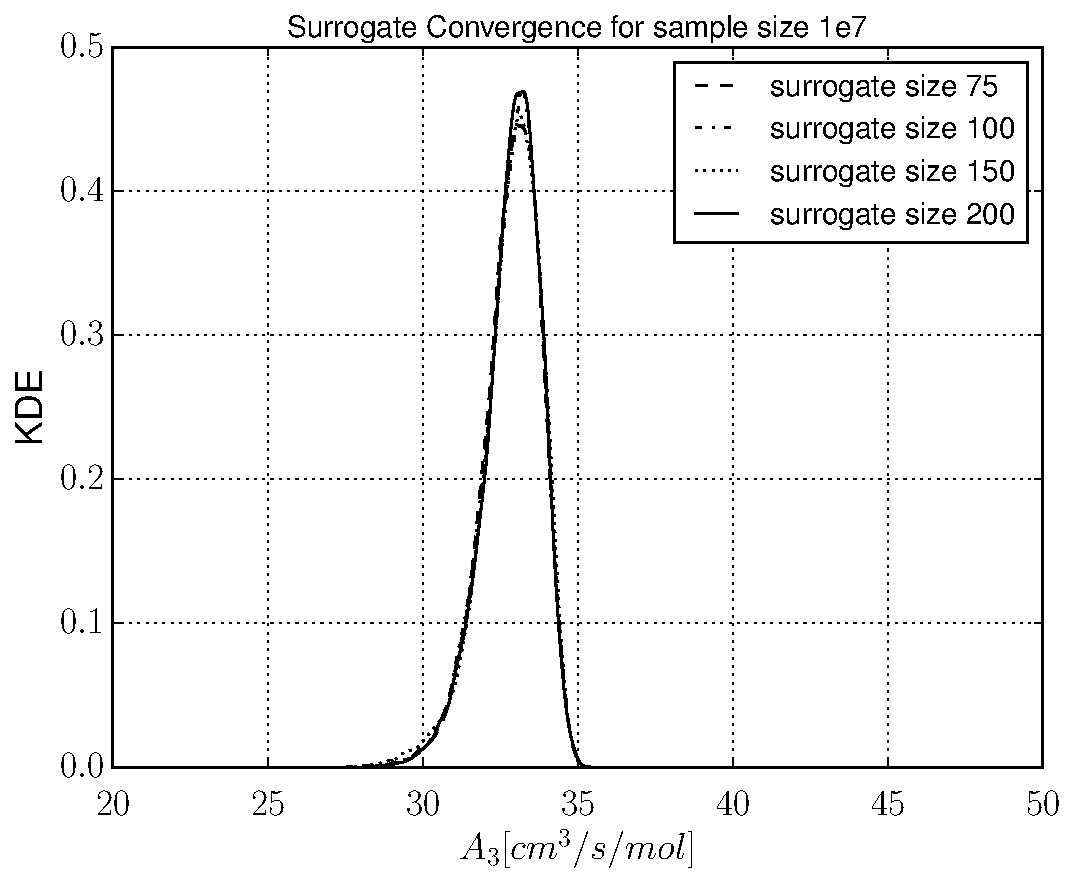
\includegraphics[scale = 0.45]{model_3/surrogate_conv_A3.pdf} 
}
\subfloat[$E_3$ surrogate convergence \label{subfig-5:surr for $E_3$}]{
			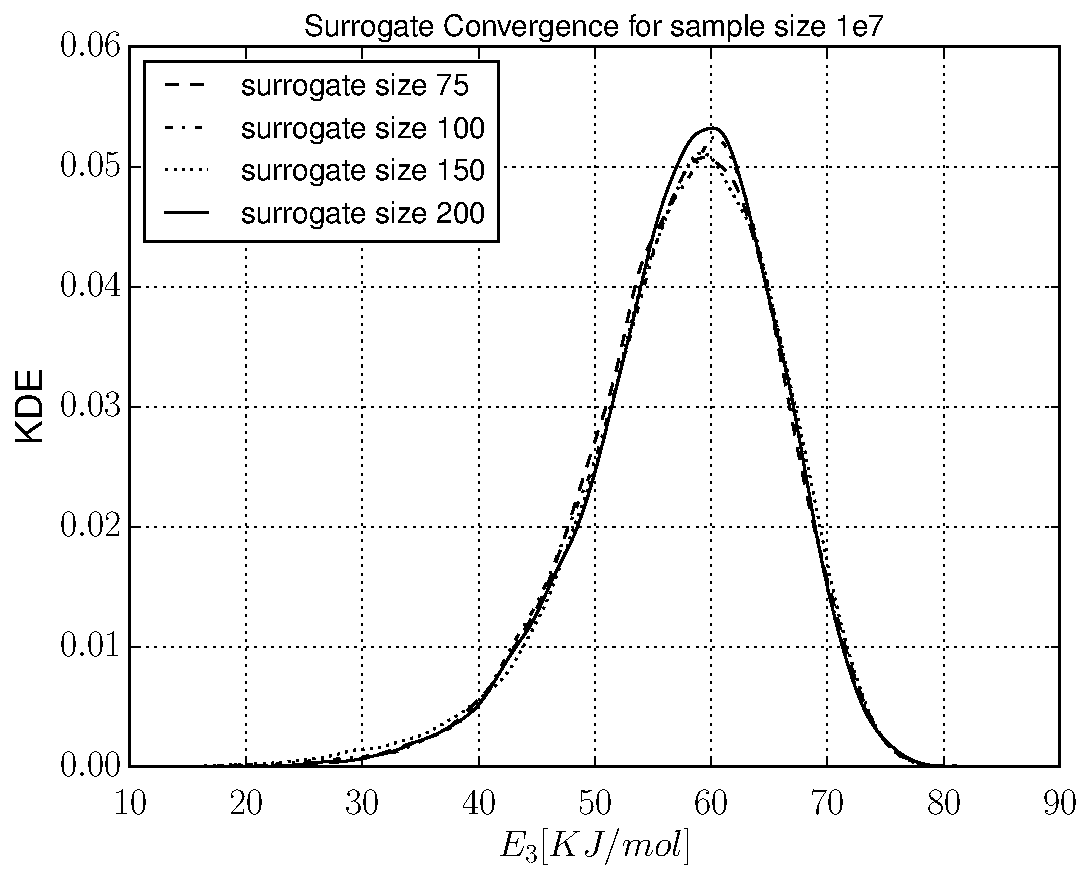
\includegraphics[scale = 0.45]{model_3/surrogate_conv_E3.pdf} 
}
\caption{Convergence for sample size 1e7 with different number of surrogate points}
}
\end{figure}


\subsection{Flamespeed Data fit}

 It is necessary to ensure that the samples of the parameter which we are drawing are fitting the flamespeed values of the experiment. In this section, we calculate the flamespeed for all the parameters drawn using the surrogate generated before. We have taken $1e7$ sample size and calculated flamespeed for different concentrations of ozone. 

\begin{figure}[H]
   \subfloat[ Flame speed for 40 \% ozone \label{subfig-1:40}]{
        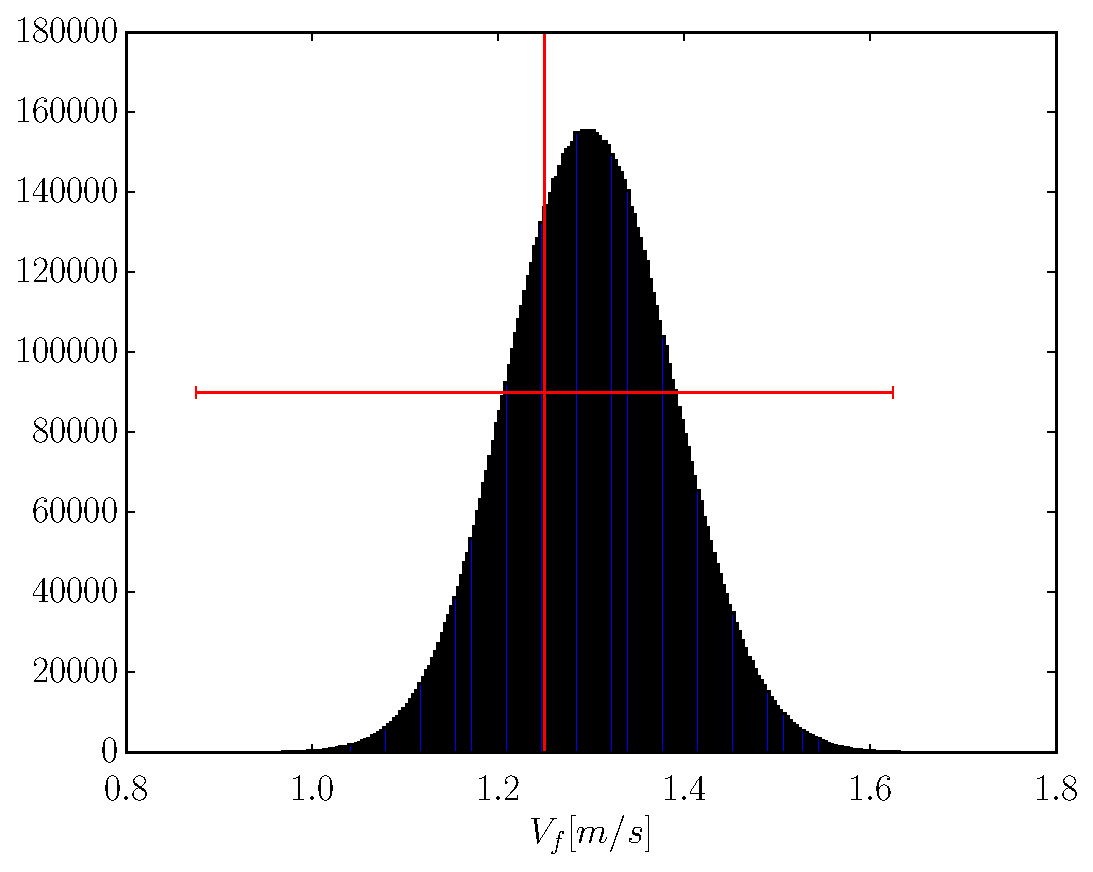
\includegraphics[scale=0.45]{model_3/flame_40.pdf}
       }
\subfloat[Flame speed for 46 \% ozone \label{subfig-2:46}]{
        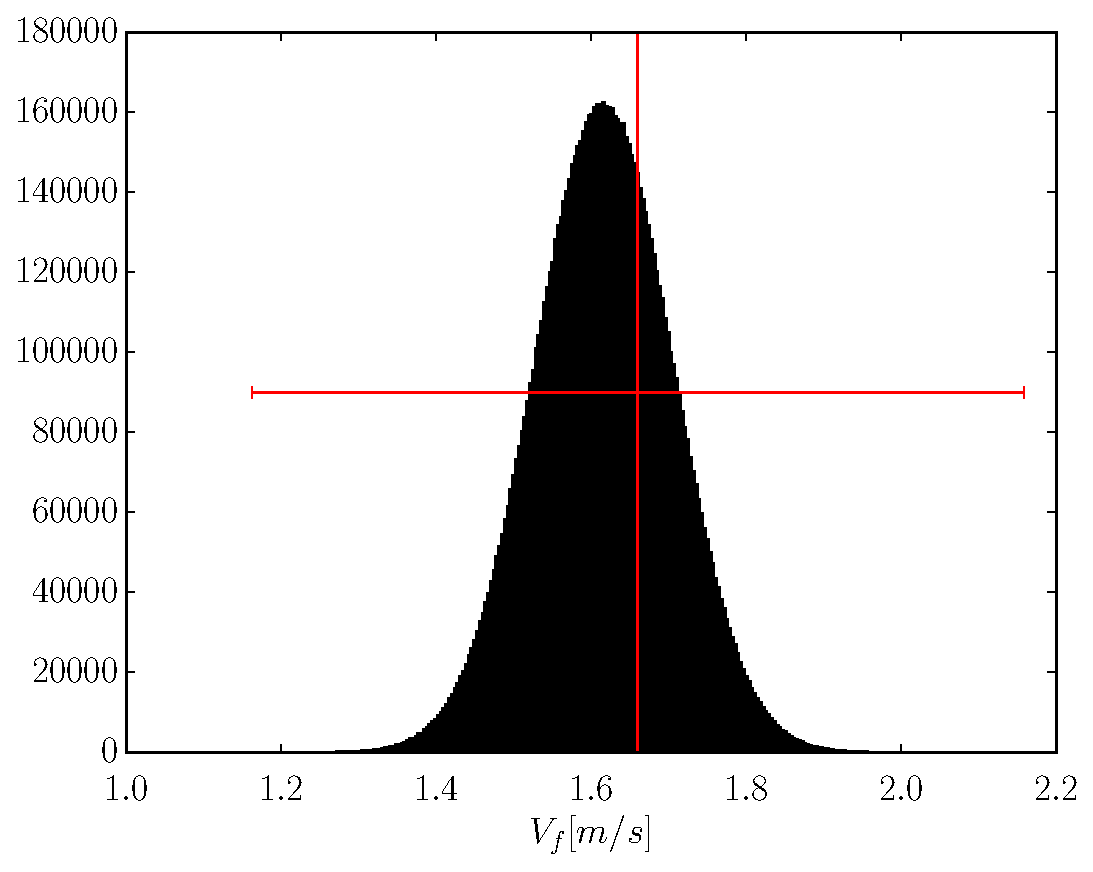
\includegraphics[scale=0.45]{model_3/flame_46.pdf}
            }
\end{figure}


 \begin{figure}[H]
  \ContinuedFloat
   \subfloat[ Flame speed for 53 \% ozone \label{subfig-3:53}]{
        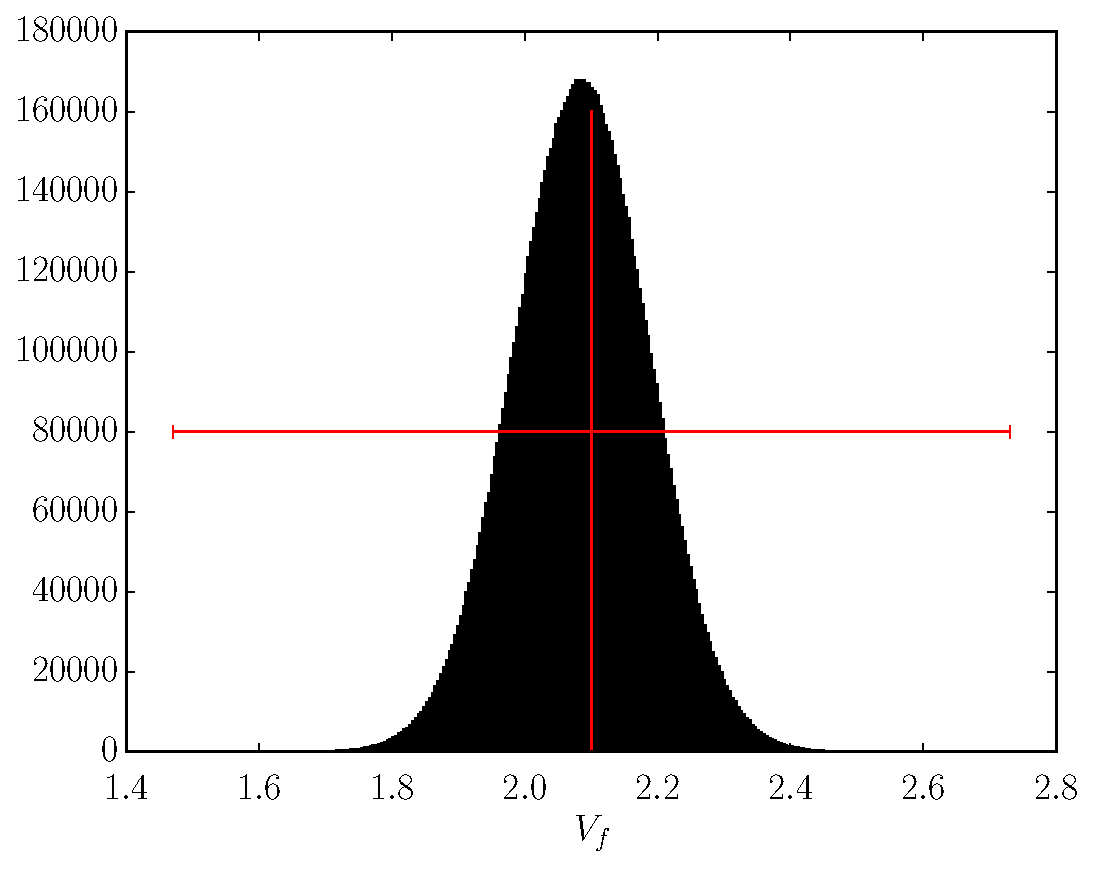
\includegraphics[scale=0.45]{model_3/flame_53.pdf}
       }
\subfloat[Flame speed for 75 \% ozone \label{subfig-4:75}]{
        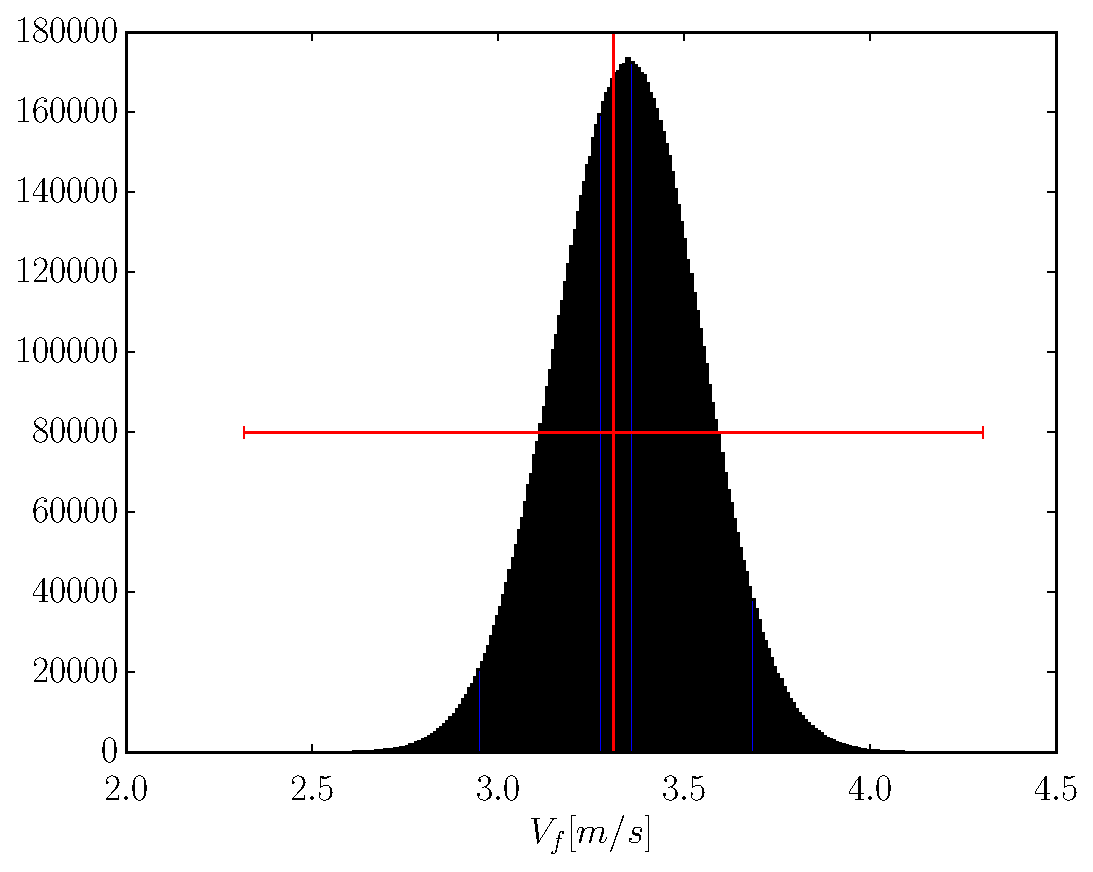
\includegraphics[scale=0.45]{model_3/flame_75.pdf}
            }
\end{figure}


 \begin{figure}[H]
  \ContinuedFloat
   \subfloat[ Flame speed for 100 \% ozone \label{subfig-5:100}]{
        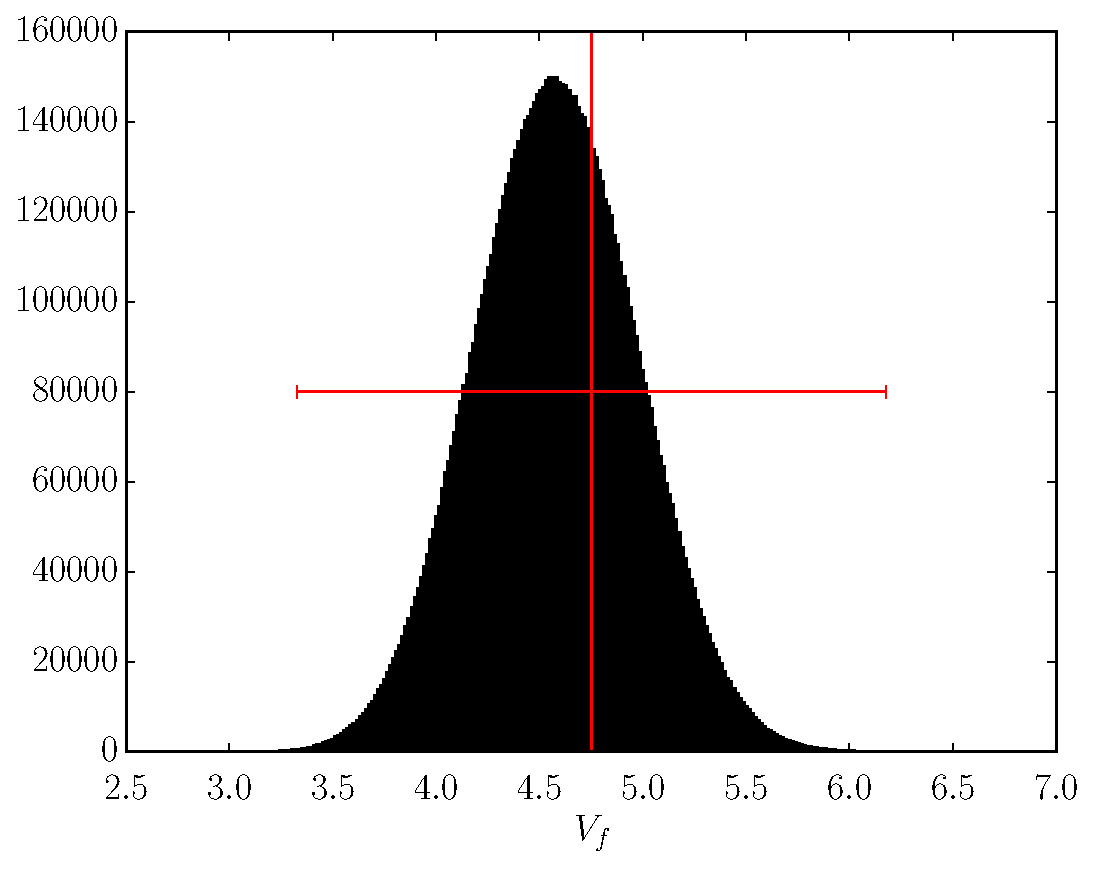
\includegraphics[scale=0.45]{model_3/flame_100.pdf}
       }
  \caption{Flamespeed Data fit}
\end{figure}



\subsection{Mean and Autocorrelation plots}

In this section, we show the mean of the samples and autocorrelation plots . The mean plot shows the initial instability due to burning period of MCMC and after that it remains constant. It shows us that we should be using atleast more than these number of samples for our analysis. The last figure shows the histogram and the various parameters of the distribution. For E3 stats: Mean:  57.5027510465, Std. Dev.:  8.36527878419, Skewness:  -0.774559635564, and Kurtosis:  1.20268267941 and for A3 stats: Mean:  32.8669085131, Std. Dev.:  0.970040786572, Skewness:  -0.961677219342, and Kurtosis:  1.79461448516.

 \begin{figure}[H]
   \subfloat[ Mean \label{subfig-1:mean}]{
        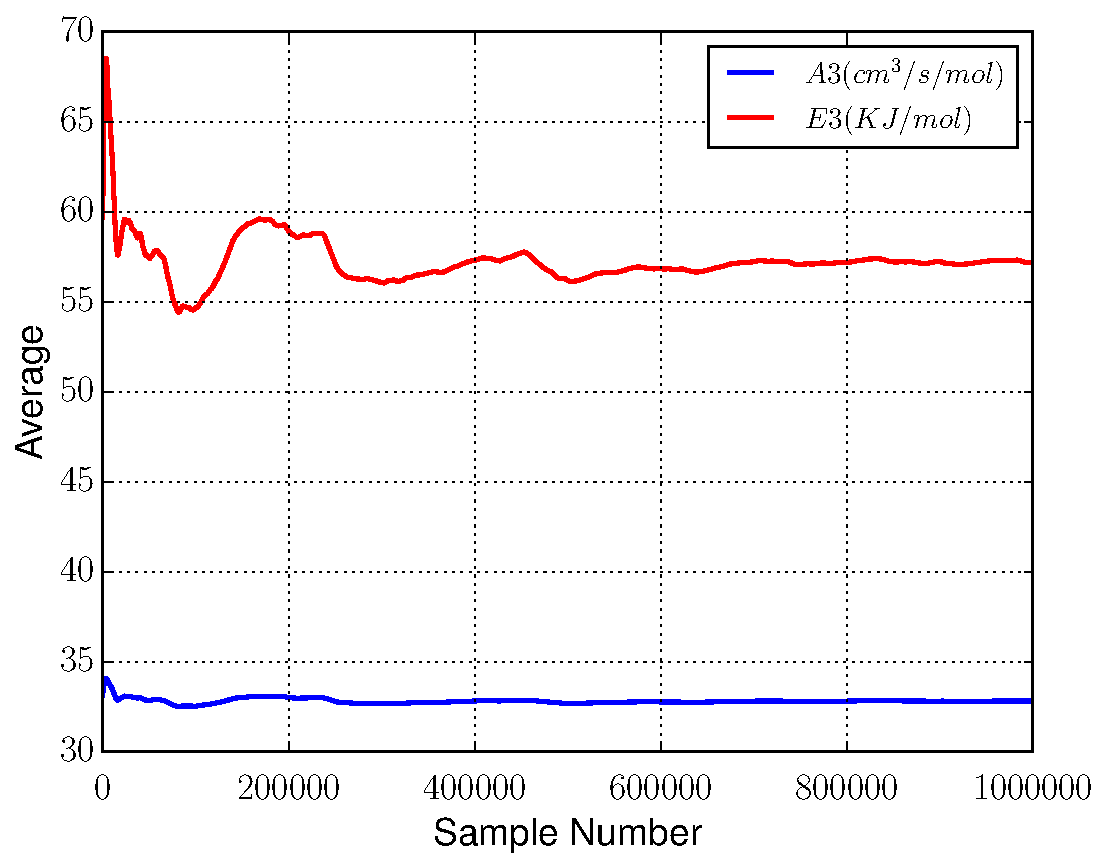
\includegraphics[scale=0.45]{model_3/M1_running_avg.pdf}
       }
\subfloat[Autocorrelation \label{subfig-2:auto}]{
        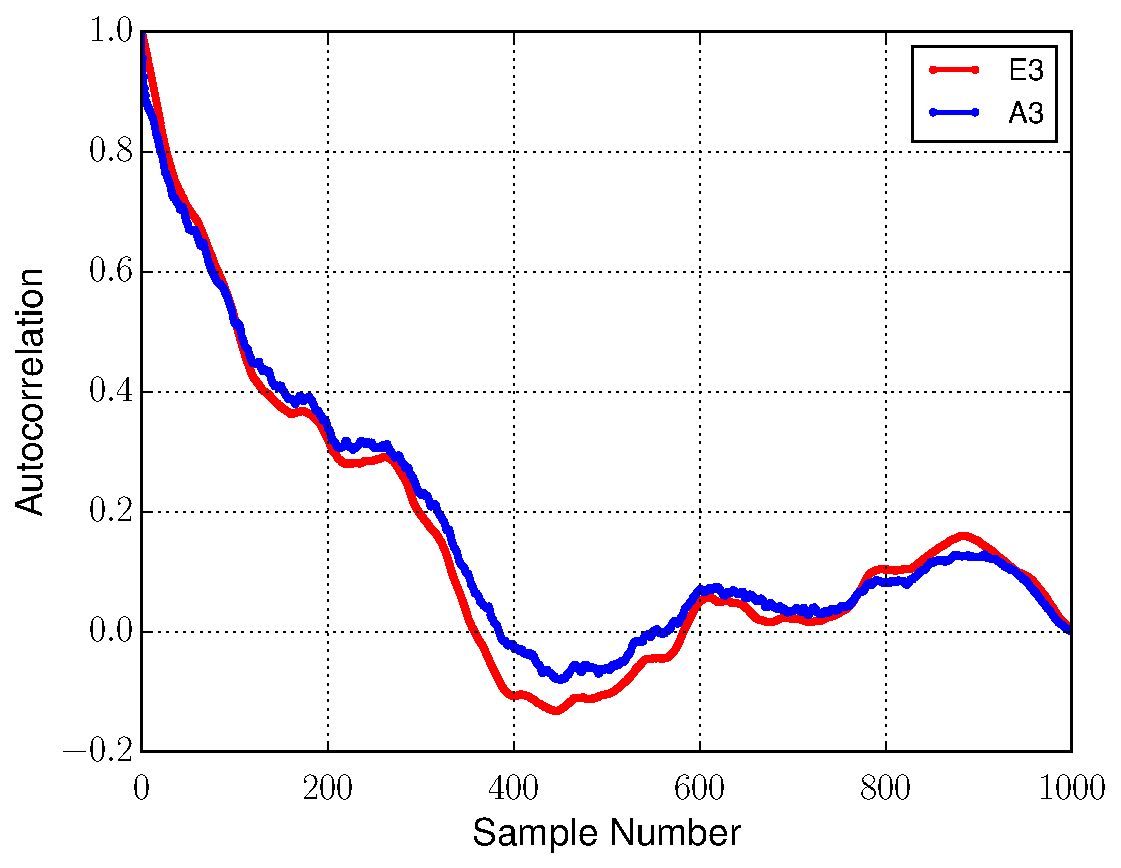
\includegraphics[scale=0.45]{model_3/M1_autocorr.pdf}
            }
            \caption{Mean and autocorrelation for sample size 1e6}
\end{figure}

 \begin{figure}[H]      
\subfloat[  $E_3$ distribution  \label{subfig-1:e3_distribution}]{
        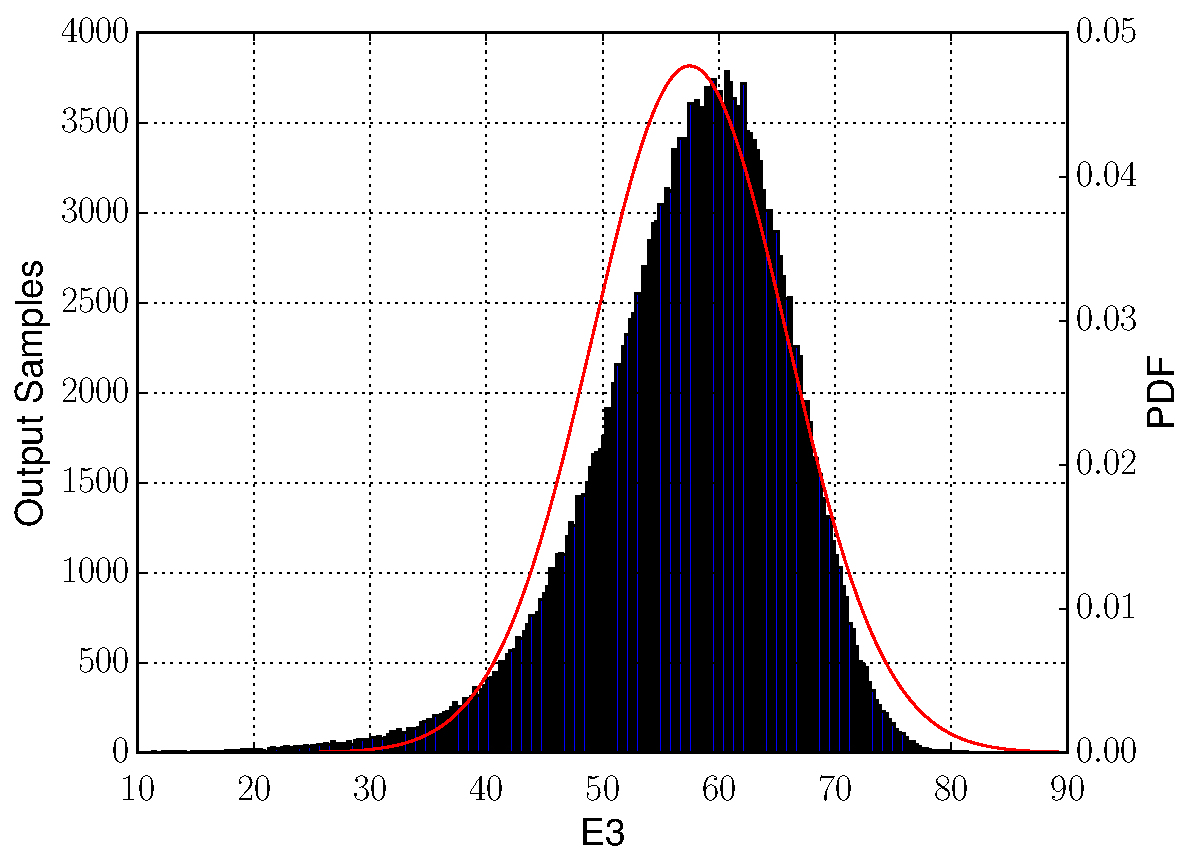
\includegraphics[scale=0.43]{model_3/E3.pdf} 
            }  
 \subfloat[ $A_3$distribution  \label{subfig-1:a3_distribution}]{
        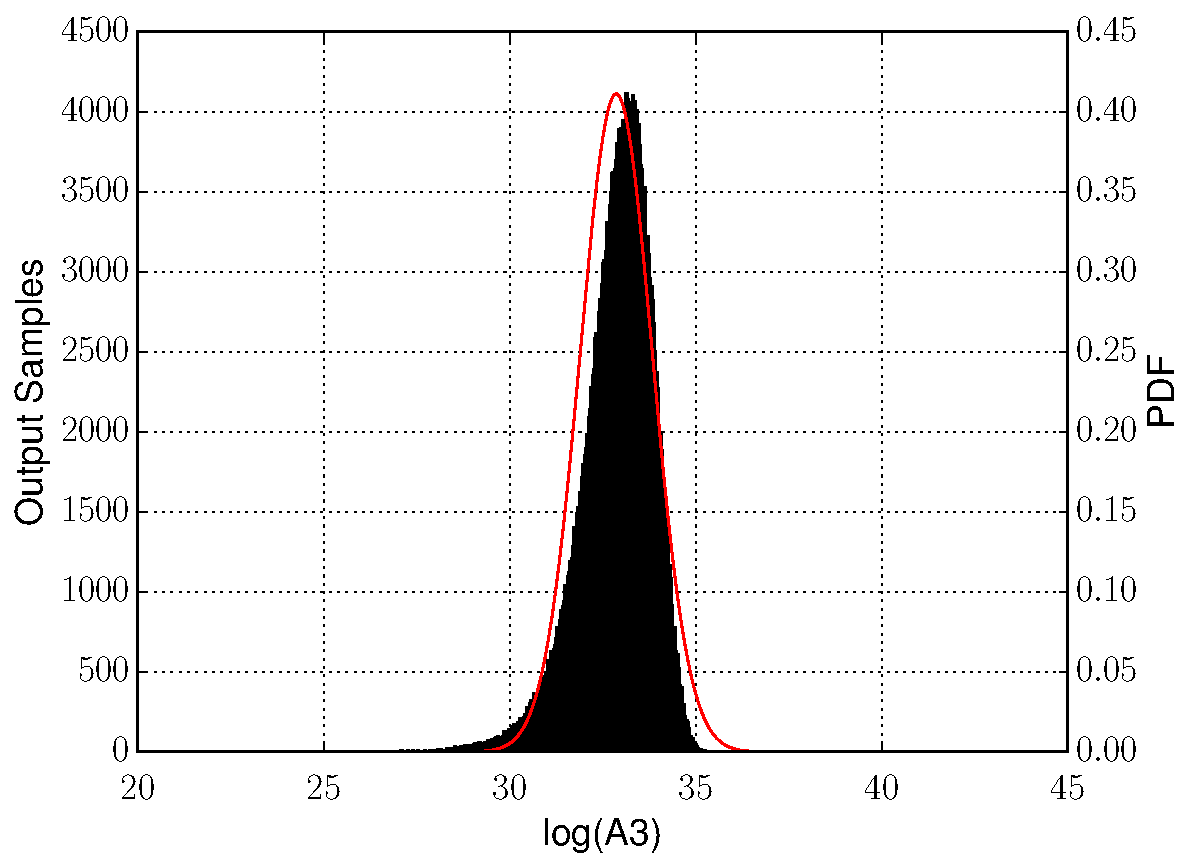
\includegraphics[scale=0.43]{model_3/A3.pdf}
            }
            \caption{$E_3$ and $A_3$ distributions}
\end{figure}
